\section{Question 3}

\begin{question}
    Using the prostate data from the faraway package in R, plot \textit{lpsa} against \textit{lcavol}. Fit the regressions of \textit{lpsa} on \textit{lcavol} and \textit{lcavol} on \textit{lpsa}. Display both regression lines on the plot.
At what point do the two lines intersect?
\end{question}

\begin{answer}
    Using the following R code to create the plot of \textit{lpsa} against \textit{lcvol}:
    \begin{verbatim}
        ## Install and library the package faraway
        #install.packages("faraway")
        library(faraway)
        ## Loading the prostate dataset from the package faraway
        data(prostate,package = "faraway")
        ## Plot lpsa against lcavol
        plot(prostate$lcavol,prostate$lpsa, xlab = "lcavol", ylab = "lpsa")
    \end{verbatim}
    , and I get the result of a plot shown in the Figure \ref{fig:fig1}.
    \begin{figure}[H]
        \centering
        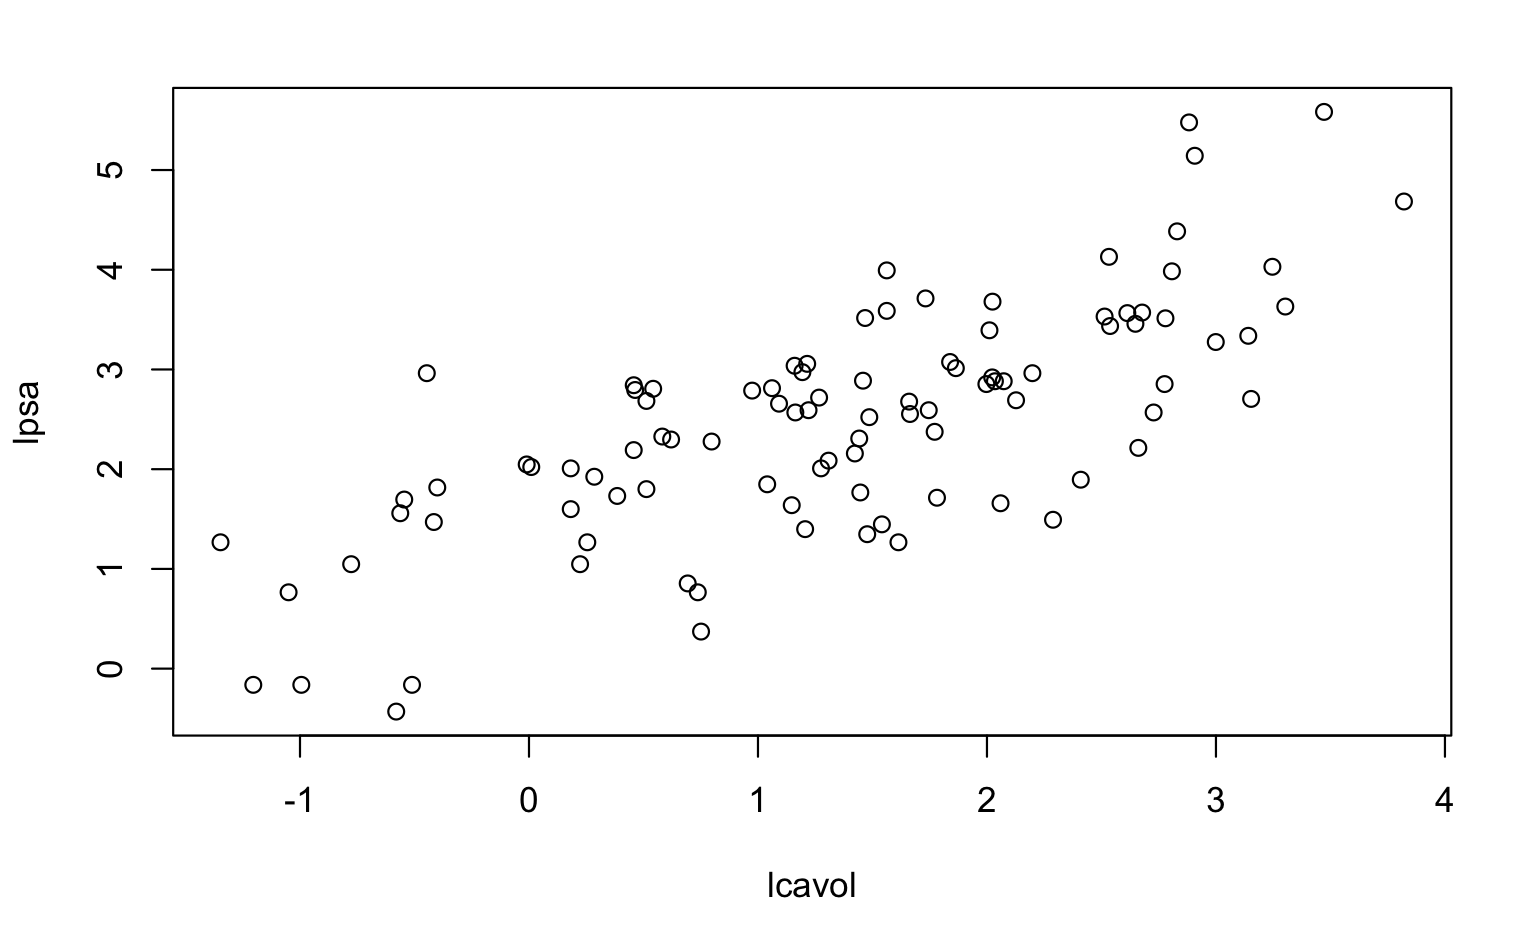
\includegraphics[width=0.8\textwidth]{Figure 1.png}
        \caption{\label{fig:fig1}plot of \textit{lpsa} against \textit{lcavol}}
    \end{figure}
    As asked in the question, I fit the regression line of the model $1$ of \textit{lpsa} on \textit{lcavol}, and fit the regression line of the model $2$ of \textit{lcavol} on \textit{lpsa}. The R code I used is the following:
    \begin{verbatim}
        ## Fit the model of lpsa on lcavol
        lm1 <- lm(prostate$lpsa~prostate$lcavol)
        ## Fit the model of lcavol on lpsa
        lm2 <- lm(prostate$lcavol~prostate$lpsa)
        ## Show the regression line of the model 1
        lm1
        ## Show the regression line of the model 2
        m2
    \end{verbatim}
    The regression line of the model $1$ is 
        \begin{align}
            \widehat{lpsa} & = 1.5073 + 0.7193\cdot lcavol \label{eqn:eqn25}
        \end{align}
    The regression line of the model $2$ is 
        \begin{align}
            \widehat{lcavol} & = -0.5086 + 0.7499\cdot lpsa \label{eqn:eqn26}
        \end{align}
    Since we want to plot both regression line onto a single plot, we want to express the second regression line in a function of \textit{lpsa}, then:    
        \begin{align}
            &\widehat{lcavol} = -0.5086 + 0.7499\cdot lpsa\\
            &\Rightarrow \widehat{lcavol} + 0.5086 = 0.7499\cdot lpsa\\
            &\Rightarrow \widehat{lpsa} = \dfrac{lcavol}{0.7499} + \dfrac{0.5086}{0.7499}\\
            &\Rightarrow \widehat{lpsa} = \dfrac{lcavol}{0.7499} + \dfrac{0.5086}{0.7499}
        \end{align}
    Using the new intercept and slope of the second regression line, I coded in R as the following:
    \begin{verbatim}
        ## Plot the regression lines
        plot(prostate$lcavol,prostate$lpsa, xlab = "lcavol", ylab = "lpsa")
        abline(lm1) 
        abline(0.5086/0.7499, 1/0.7499)
    \end{verbatim}
    The plot I obtained is shown in the Figure \ref{fig:fig2}.
    \begin{figure}[H]
        \centering
        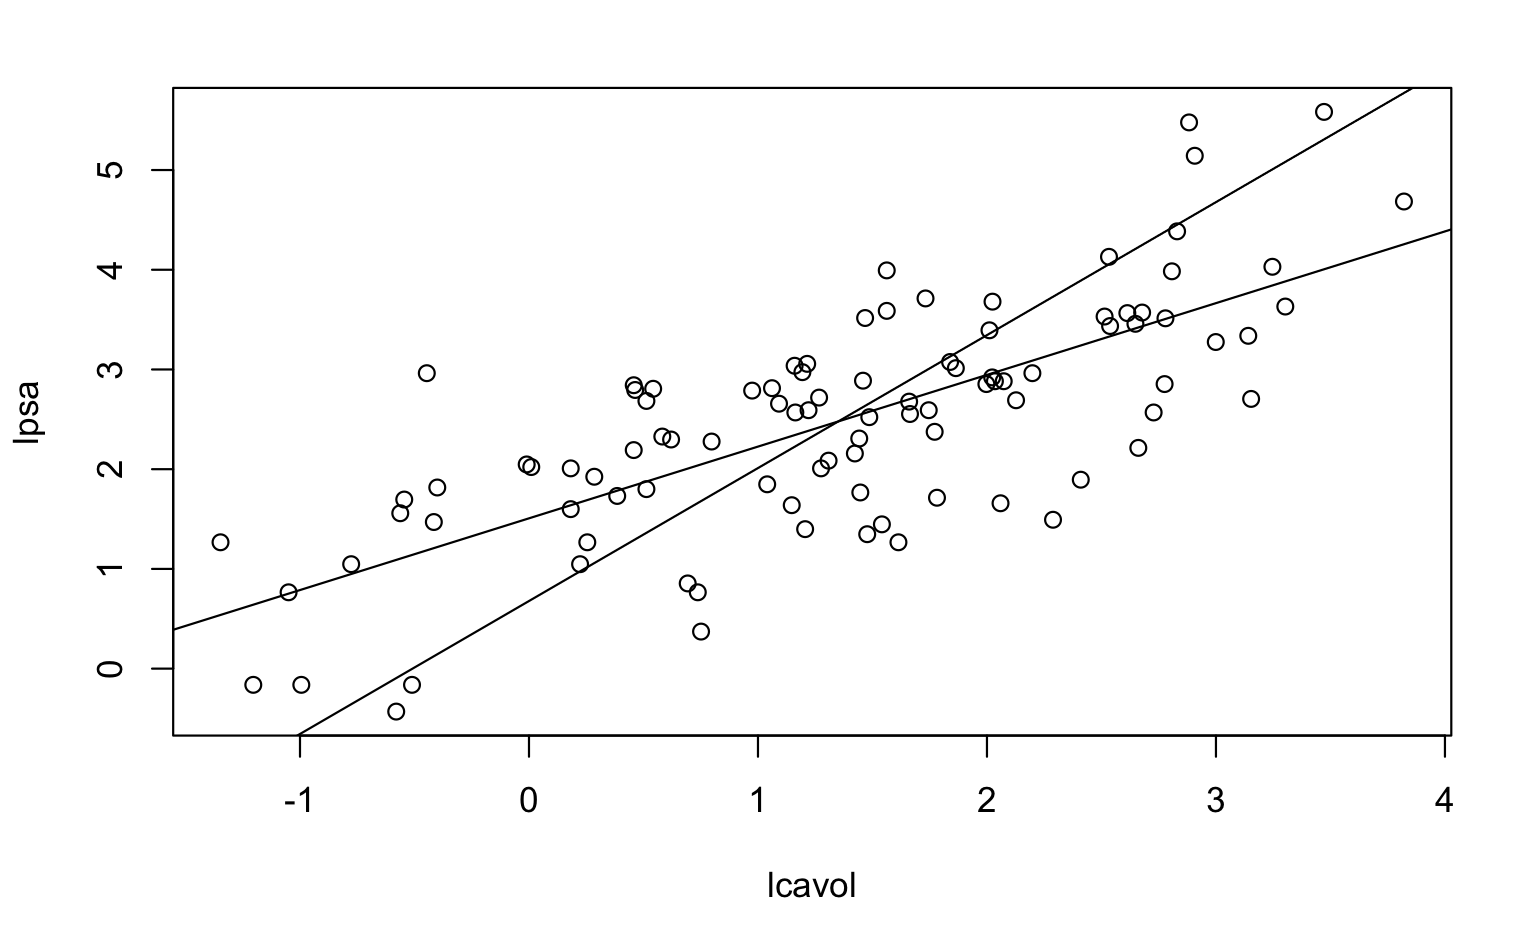
\includegraphics[width=0.8\textwidth]{Figure 2.png}
        \caption{\label{fig:fig2}plot with both regression lines}
    \end{figure}
    In order the find the point of intersection of the both regression lines, we should create a system of equation using equation (\ref{eqn:eqn25}) and equation (\ref{eqn:eqn26}). Solve the system of equation, we have the point of intersection, which is $(1.34982,2.47823)$
\end{answer}